% =============================================
% =============================================
% Document class: Article
\documentclass[ a4paper, twoside, 11pt]{article}
% Packages: LaTeX (Depth-1)
\usepackage[ vlined, linesnumbered, ruled]{algorithm2e}
\usepackage{ amsfonts, amsmath, amssymb, amsthm}
\usepackage[ titletoc, title]{appendix}
\usepackage{ bbm}
\usepackage{ color}
\usepackage{ dsfont}
\usepackage{ enumitem}
\usepackage{ graphicx}
\usepackage{ fancyhdr, float, fullpage}
\usepackage{ hyperref}
\usepackage{ lastpage, latexsym, lipsum}
\usepackage{ mathrsfs, mathtools, multicol}
\usepackage{ parskip}
\usepackage{ setspace, stmaryrd, subcaption}
\usepackage{ tabularx}
\usepackage{ wasysym}
\usepackage[ dvipsnames, table]{ xcolor}
\usepackage{ xfrac}
% Packages: LaTeX (Depth-2)
\usepackage{ epstopdf}

% =============================================
\topmargin 			= -1.6cm
\headheight 		= .90cm
\headsep 			= .80cm
\textheight 		= 24.0cm
\textwidth 			= 15.5cm
\oddsidemargin		= 0.cm
\evensidemargin 	= 0.cm

% =============================================
% =============================================
% Macros: Language
\newcommand{\define}{\triangleq}
\newcommand{\done}{\hfill $\square$}
%\newcommand{\eqCIRC}{\stackrel{\circ}{=}}
%\newcommand{\eqSTAR}{\stackrel{*}{=}}
\renewcommand{\epsilon}{\varepsilon}
\newcommand{\eg}{\textit{e.g.,\;}}
\newcommand{\egc}{\textit{e.g.:\;}}
\newcommand{\Eg}{\textit{E.g.,\;}}
\newcommand{\Egc}{\textit{E.g.:\;}}
\newcommand{\ie}{\textit{i.e.,\;}}
\newcommand{\iec}{\textit{i.e.:\;}}
\newcommand{\Ie}{\textit{I.e.,\;}}
\newcommand{\Iec}{\textit{I.e.:\;}}
\newcommand{\QED}{\hfill $\blacksquare$}
\renewcommand{\tilde}[1]{\widetilde{#1}}
\newcommand{\tsup}[1]{\ensuremath{^{\text{#1}}}}
\newcommand{\tsub}[1]{\ensuremath{_{\text{#1}}}}
\renewcommand{\vec}[1]{{\boldsymbol{#1}}}

% Macros: Optimization & Probability
\DeclareMathOperator*{\argmax}{arg\,max}
\DeclareMathOperator*{\argmin}{arg\,min}
\newcommand{\Exp}{\mathbb{E}}
\newcommand{\Indicate}[1]{ \IndFun \, \{ \, #1 \, \} }
\renewcommand{\Pr}{\mathbb{P}}
\newcommand{\Normal}{\mathcal{N}}
\newcommand{\std}{\text{std}}
\newcommand{\var}{\text{var}}

% Macros: Sets
\newcommand{\Complex}{\mathbb{C}}
\renewcommand{\emptyset}{\varnothing}
\newcommand{\Nat}{\mathbb{N}}
\renewcommand{\Re}{\mathbb{R}}
\newcommand{\ReNN}{{\Re}_{\geq 0}}
\newcommand{\ReSP}{{\Re}_{> 0}}
\renewcommand{\subset}{\subseteq}
\renewcommand{\supset}{\supseteq}
\newcommand{\Z}{\mathbb{Z}}
\newcommand{\ZNN}{{\Z}_{\geq 0}}

% Macros: Spacing & Other Commands
\newcommand{\fullcut}{\vspace{-\baselineskip}}
\newcommand{\fullskip}{\vspace{\baselineskip}}
\newcommand{\halfcut}{\vspace{-0.5\baselineskip}}
\newcommand{\halfskip}{\vspace{0.5\baselineskip}}
\renewcommand{\figurename}{Figura}
\renewcommand{\tablename}{Tabla}

% =============================================
% Sesion de Clase
\newcommand{\sesion}{02}
% Macros para definiciones, teoremas, etc
\newcounter{sesion}
\setcounter{sesion}{\sesion}
\theoremstyle{definition}
\newtheorem{definition}{Definici\'on}[sesion]
\newtheorem{example}[definition]{Ejemplo}
\newtheorem{exercise}[definition]{Ejercicio}
\newtheorem{note}[definition]{Nota}
\newtheorem{problem}[definition]{Problema}
\newtheorem{theorem}[definition]{Teorema}

% =============================================
% =============================================
\newcommand{\HeaderLine}{}
\newcommand{\FooterLine}{P\'agina \thepage ~de \pageref*{LastPage}}

\pagestyle{fancyplain}
\fancyhf{}

\rhead[]{\fancyplain{}{\HeaderLine}}
\lhead[\fancyplain{}{\HeaderLine}]{}
\lfoot[\fancyplain{}{\FooterLine}]{}
\rfoot[]{\fancyplain{}{\FooterLine}}

\renewcommand{\headrulewidth}{0.4pt}
\renewcommand{\footrulewidth}{0.4pt}
\renewcommand{\thefootnote}{\fnsymbol{footnote}}

% =============================================
% =============================================
\begin{document}
\allowdisplaybreaks

\begin{center}
\Large Control Autom\'atico: Lecci\'on \sesion \\[0.5ex]
\small \textbf{A\~no:} 2016-2017 \qquad \textbf{T\'ermino:} II \qquad
\textbf{Instructor:} Luis I. Reyes Castro \qquad \textbf{Paralelo:} 02
\end{center}
\halfskip

\fbox{

\begin{minipage}[b][\height][t]{\textwidth}
\vspace{0.2 cm}

\begin{center}
\textbf{COMPROMISO DE HONOR}
\end{center}
\vspace{0.4 cm}

\scriptsize
{
Yo, \rule{60mm}{.1pt} al firmar este compromiso, reconozco que la presente lecci\'on est\'a dise\~nada para ser resuelta de manera individual, que puedo usar un l\'apiz o pluma y una calculadora cient\'ifica, \linebreak que solo puedo comunicarme con la persona responsable de la recepci\'on de la lecci\'on, y que cualquier instrumento de comunicaci\'on que hubiere tra\'ido debo apagarlo. Tambi\'en estoy conciente que no debo consultar libros, notas, \linebreak ni materiales did\'acticos adicionales a los que el instructor entregue durante la lecci\'on o autorice a utilizar. Finalmente, me comprometo a desarrollar y presentar mis respuestas de manera clara y ordenada. \\

Firmo al pie del presente compromiso como constancia de haberlo le\'ido y aceptado. 
\vspace{0.4 cm}

Firma: \rule{60mm}{.1pt} \qquad N\'umero de matr\'icula: \rule{40mm}{.1pt} \hspace{0.5cm} \\[-0.8ex]

}

\end{minipage}

}
\vspace{\baselineskip}

%% =============================================
%\begin{problem}
%Suponga que usted se encuentra analizando un sistema descrito por la \linebreak siguiente ecuaci\'on diferencial, la cual relaciona la se\~nal de entrada o referencia $r(t)$ con la se\~nal de salida o variable controlada $c(t)$. 
%\[
%\frac{d^2c(t)}{dt^2} + 6 \, \frac{dc(t)}{dt} + 8 \, c(t) 
%\; = \; \frac{1}{3} \, \frac{dr(t)}{dt} + r(t)
%\]
%Con esto en mente, encuentre: 
%\begin{itemize}
%\item \textbf{[1 Punto]} La funci\'on de transferencia $G(s) = C(s)/R(s)$. 
%%\[
%%G(s)
%%\; = \; \frac{(1/3)s + 1}{s^2 + 6s + 8}
%%\; = \; \frac{1}{3} \, \frac{s+3}{s^2 + 6s + 8}
%%\; = \; \frac{1}{3} \, \frac{s+3}{(s+2)(s+4)}
%%\]
%\item \textbf{[2 Puntos]} La respuesta de la salida $c(t)$ cuando la entrada $r(t)$ es un escal\'on. 
%%\[
%%c(t) \; = \; 
%%\left(
%%\frac{3}{24}
%%- \frac{1}{12} \, e^{-2t}
%%- \frac{1}{24} \, e^{-4t}
%%\right) \, u(t)
%%\]
%\end{itemize}
%
%\end{problem}
%\vspace{\baselineskip}

%% =============================================
%\begin{problem}
%Considere la siguiente funci\'on de transferencia: 
%\[
%G(s) \; = \; \frac{s + 2}{s^2 + 4s + 20}
%\]
%Encuentre: 
%\begin{itemize}
%\item \textbf{[1 Punto]} La ecuaci\'on diferencial del sistema que coresponde a $G(s)$. 
%\item \textbf{[2 Puntos]} La respuesta de la salida $c(t)$ cuando la entrada $r(t)$ es un impulso.  
%\end{itemize}
%
%\end{problem}
%\vspace{\baselineskip}

% =============================================
\begin{problem}
Considere el siguente modelo de la suspensi\'on de un autom\'ovil.  
\begin{figure}[htb]
\centering
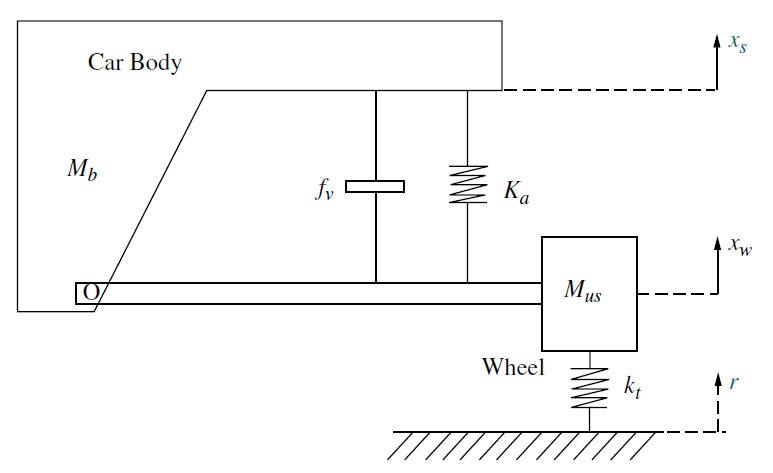
\includegraphics[ width = 0.5\textwidth]{fig_P2-36.jpg}
\end{figure}

Encuentre la funci\'on de transferencia $G(s) \define X_s(s) / R(s)$ que relaciona la perturbaci\'on de la carretera $r(t)$ con el desplazamiento vertical del cuerpo del veh\'iculo $x_s(t)$. \textbf{[5 Puntos]}

\emph{Soluci\'on:} Escribiendo la sumatoria de fuerzas en la rueda (cuya masa es $M_{us}$) y en el cuerpo del autom\'ovil (cuya masa es $M_{b}$) obtenemos el siguiente par de ecuaciones diferenciales: 
\begin{align*}
M_{us} \, \ddot{x}_w(t) \; & = \; 
-k_t \, ( x_w(t) - r(t) ) + K_a \, ( x_s(t) - x_w(t) ) 
+ f_v \, ( \dot{x}_s(t) - \dot{x}_w(t) ) \\
M_{b} \, \ddot{x}_s(t) \; & = \; 
-K_a \, ( x_s(t) - x_w(t) ) 
- f_v \, ( \dot{x}_s(t) - \dot{x}_w(t) )
\end{align*}
Tomando la Transformaci\'on de Laplace de ambos lados de ambas ecuaciones y organizando los t\'erminos resultantes obtenemos el siguiente par de ecuaciones algebraicas: 
\begin{align*}
( \, M_{us} \, s^2 + f_v \, s + ( k_t + K_a ) \, ) \, X_w(s) 
- ( \, f_v \, s + K_a \, ) \, X_s(s) \; & = \; k_t \, R(s) \\
( \, M_{b} \, s^2 + f_v \, s + K_a \, ) \, X_s(s) 
- ( \, f_v \, s + K_a \, ) \, X_w(s) \; & = \; 0
\end{align*}
Resolviendo para $X_w(s)$ en la segunda ecuaci\'on, obtenemos: 
\[
X_w(s) \; = \; 
\left( \frac{  M_{b} \, s^2 + f_v \, s + K_a }{ f_v \, s + K_a } \, \right) \, X_s(s)
\]
Luego, reemplazando $X_w(s)$ en la primera ecuaci\'on por la expresi\'on anterior obtenemos: 
\[
\left[ \frac{ ( \, M_{us} \, s^2 + f_v \, s + ( k_t + K_a ) \, ) \, ( \, M_{b} \, s^2 + f_v \, s + K_a \, ) }{ f_v \, s + K_a } - ( \, f_v \, s + K_a \, ) \, \right] \, X_s(s) \; = \; k_t \, R(s)
\]
Finalmente, vemos que: 
\[
G(s) \; = \; \frac{ k_t \, ( \, f_v \, s + K_a \, ) }{ ( \, M_{us} \, s^2 + f_v \, s + ( k_t + K_a ) \, ) \, ( \, M_{b} \, s^2 + f_v \, s + K_a \, ) - ( \, f_v \, s + K_a \, )^2 }
\]

\emph{Opcional:} Si denotamos al denominador de $G(s)$ como $D(s)$ entonces: 
\begin{align*}
D(s) \; & = \; ( \, M_{us} \, M_b \, ) \, s^4 + ( \, M_{us} + M_b \, ) \, f_v \, s^3 \\ & + ( \, M_{us} \, K_a + M_b \, ( k_t + K_a ) \, ) \, s^2 + f_v \, k_t \, s + ( \, k_t + K_a \, )
\end{align*}

\end{problem}
\vspace{\baselineskip}

% =============================================
\begin{problem}
Considere el siguente circuito anal\'ogico.  
\begin{figure}[htb]
\centering
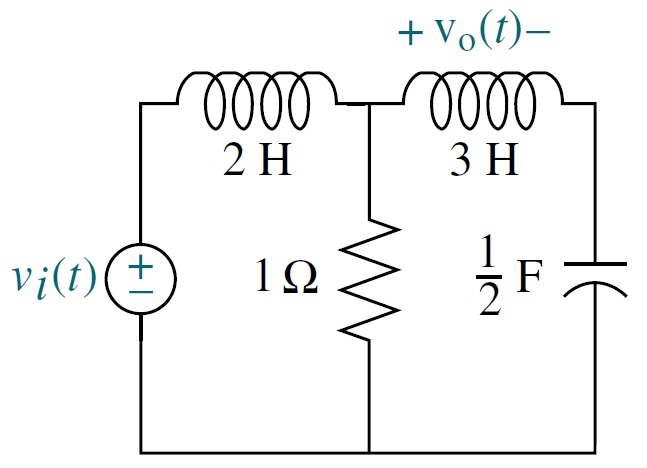
\includegraphics[ width = 0.35\textwidth]{fig_P2-5a.jpg}
\end{figure}

Encuentre la funci\'on de transferencia $G(s) \define V_o(s) / V_i(s)$ que relaciona el voltage en la fuente $v_i(t)$ con el voltage $v_o(t)$ a trav\'es del inductor se\~nalado en la figura. \textbf{[5 Puntos]}

\emph{Soluci\'on:} Primero introducimos la corriente transformada $I_1(s)$ en el lazo de la izquierda en el sentido de las manecillas del reloj, junto con la corriente transformada $I_2(s)$ en el lazo de la derecha en el mismo sentido que la primera corriente. Luego reemplazamos el inductor de \linebreak $L = 2$ H por una impedancia de $Z(s) = 2s$, el inductor de $L = 3$ H por una impedancia de $Z(s) = 3s$, la resistencia de $R = 1$ $\Omega$ por una impedancia $Z(s) = 1$, y el capacitor de \linebreak $C = 1/2$ F por una impedancia de $Z(s) = 2/s$. 

Ahora, sumando voltajes alrededor del lazo de la izquierda, obtenemos: 
\begin{align*}
& V_i(s) - (2s) \, I_1(s) - (1) \, ( I_1(s) - I_2(s) ) \; = \; 0 \\
& \Longrightarrow \; 
V_i(s) \; = \; ( 2s + 1 ) \, I_1(s) - I_2(s)
\end{align*}
Mas a\'un, sumando voltajes alrededor del lazo de la derecha, obtenemos: 
\begin{align*}
& - (1) \, ( I_2(s) - I_1(s) ) - (3s) \, I_2(s) - \left( \frac{2}{s} \right) I_2(s) \; = \; 0 \\
& \Longrightarrow \; 
I_1(s) \; = \; \left( \, 1 + 3s + \frac{2}{s} \, \right) I_2(s) \\
& \Longrightarrow \; 
I_1(s) \; = \; \left( \, \frac{ 3s^2 + s + 2 }{s} \, \right) I_2(s)
\end{align*}
A su vez, reemplazando $I_1(s)$ por la expresi\'on anterior en la ecuaci\'on del lazo de la izquierda, vemos que: 
\begin{align*}
& V_i(s) \; = \; 
\left[ \, \frac{ ( 2s + 1 ) \, ( 3s^2 + s + 2 ) }{s} - 1 \, \right] I_2(s) \\
& \Longrightarrow \; 
V_i(s) \; = \; 
\left( \, \frac{ 6 \, s^3 + 5 \, s^2 + 4 \, s + 2 }{s} \, \right) I_2(s)
\end{align*}
Finalmente, reconociendo que $V_o(s) = (3s) \, I_2(s)$, concluimos que: 
\begin{align*}
& V_i(s) \; = \; 
\left( \, \frac{ 6 \, s^3 + 5 \, s^2 + 4 \, s + 2 }{3s^2} \, \right) V_o(s) \\
& \Longrightarrow \; G(s) \; = \; 
\frac{ 3 \, s^2 }{ 6 \, s^3 + 5 \, s^2 + 4 \, s + 2 }
\end{align*}

\end{problem}
\vspace{\baselineskip}

\end{document}
